\documentclass[letterpaper, 11pt]{article} 

\usepackage{graphics,graphicx}
\usepackage{multicol} 
\usepackage{parskip}
\usepackage{amsmath}
\usepackage{multirow}
\usepackage[utf8]{inputenc}
\usepackage{fancyhdr}
\usepackage[title]{appendix}
\usepackage{wasysym}
\usepackage{url}
\usepackage{subcaption}
\usepackage{advdate}

\usepackage[font=footnotesize,labelfont=small]{caption}
\captionsetup{width=0.85\linewidth}

\RequirePackage{geometry}
\geometry{margin=2cm}

\setlength{\parskip}{0.2cm}
\setlength{\parindent}{0pt}

\usepackage{listings}
\usepackage{xcolor}

\definecolor{codegreen}{rgb}{0,0.6,0}
\definecolor{codegray}{rgb}{0.5,0.5,0.5}
\definecolor{codepurple}{rgb}{0.58,0,0.82}
\definecolor{backcolour}{rgb}{0.95,0.95,0.92}

\lstdefinestyle{mystyle}{
	backgroundcolor=\color{backcolour},   
	commentstyle=\color{codegreen},
	keywordstyle=\color{magenta},
	numberstyle=\tiny\color{codegray},
	stringstyle=\color{codepurple},
	basicstyle=\ttfamily\footnotesize,
	breakatwhitespace=false,         
	breaklines=true,                 
	captionpos=b,                    
	keepspaces=true,                 
	numbers=left,                    
	numbersep=5pt,                  
	showspaces=false,                
	showstringspaces=false,
	showtabs=false,                  
	tabsize=2
}

\lstset{style=mystyle}


\title{Assignment 2: Multithreading and Solving System of Linear Equations Algorithms}
\author{
Tai Duc Nguyen \\
ECEC 622: Parallel Computer Architecture
}
\date{\AdvanceDate[-1]\today}

\begin{document}

\maketitle

\rule{\textwidth}{1pt}

\begin{abstract}
	Knowledge from the previous assignment about multithreading's quirks and benefits is leveraged to develop a common algorithm used in solving system of linear equations called Iterative Jacobian Solver. 
\end{abstract}

\rule{\textwidth}{1pt}

\section{Experimental Setup}

The Jacobi method is an iterative algorithm for determining the solutions of a strictly diagonally dominant system of linear equations ($A\boldsymbol{x}=B$). Each diagonal element is solved for, and an approximate value is plugged in. The process is then iterated until it converges. This algorithm is a stripped-down version of the Jacobi transformation method of matrix diagonalization.

The multithreaded version of this algorithm is implemented as follows:

\begin{lstlisting}
	Create a copy of matrix X called new_X
	Initialize barrier sync
	
	Create threads
	Reserve memory for partial SSDs (sum of the squared differences)
	Allocate memory on heap for threads' data
	
	Start all threads. For each thread:
		while not DONE:
			Each thread is a assigned a row i;
				The vector dot product of A[i,:] with X is computed and stored in variable sum;
				new_X[i] = (B[i] - sum)/A[i,i];
				
				tmp_ssd = X[i] - new_X[i];
				prt_ssd += tmp_ssd * tmp_ssd;
				
				i += num_threads (striding method)
			partial_ssd[thread_id] = prt_ssd
			
			BARRIER SYNC
			
			if thread_id is 0:
				sum up all partial ssds;
				if sqrt(sum_ssds) < TOLERANCE:
					DONE = 1;
			
			BARRIER SYNC
			
			if not DONE:
				Swap X and new_X;
		
	Stop all threads


\end{lstlisting}

\textit{Note: running \texttt{make all} will generate the report in \texttt{rpt.txt}}

\section{Experimental Result}

\begin{figure}[htb!]
	\centering
	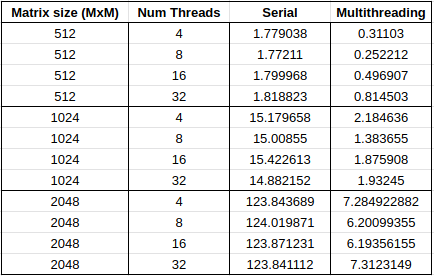
\includegraphics[width=0.6\linewidth]{results.png}
	\caption{Results of execution times in seconds of the serial vs the multithreaded version using the pthread interface}
	\label{fig1}
\end{figure}

\section{Discussion}

From Figure \ref{fig1}, it is apparent that the larger the problem size, multithreading provides increasingly significant improvements ($\approx$ 6x for 512, $\approx$ 10x for 1024 and $\approx$ 17x for 2048). This result can be improved with better memory management, better memory access pattern, and, better initial approximation of X (this can vastly reduce the number of iterations needed to reach the tolerance limit).
From the data, it is also shown that 8 threads provide the best amount of speed up. Having more than 8 threads will increase the amount of overhead and make the program runs slower.

\end{document}